\documentclass{beamer}

\usepackage{amsfonts,amsmath,comment,graphicx}

\title{Spectral Rigid Body Dynamics}
\author{Mikola Lysenko}

\begin{document}

\newcommand{\R}{\mathbb{R}}

\maketitle

\section{Rigid Body Dynamics}

\begin{frame}
\frametitle{Rigid Body Dynamics}
An approximate model of low energy physics for stiff objects

\pause
\vskip15pt
Pros:
\begin{itemize}
	\item{+} Pretty accurate at human energy scales
	\item{+} Good for stiff materials (ie metals, plastics etc.)
	\item{+} Easy kinematic constraints (useful for mechanisms)
	\item{+} Standard animation tool (videogames!)
\end{itemize}

\pause
\vskip15pt
Cons:
\begin{itemize}
	\item{-} Inaccurate at extremely large energies
	\item{-} Bad for materials with low elastic modulus
	\item{-} Not always solvable! (See: Painleve's paradox)
\end{itemize}
\end{frame}

\begin{frame}
\frametitle{What is a Rigid Body?}
An idealized solid object with elastic modulus $= \infty$
\pause
\vskip5pt
We identify a body $B$ with a scalar field, $\varphi : \R^d \to \R^+$
\vskip5pt
\begin{center}

\includegraphics[height=1.1in]{figures/massfield.png}
\end{center}
\vskip5pt
$\varphi$ represents the mass distribution of $B$
\vskip5pt
$\varphi(x) = 0$ indicates $B$ does not occupy the space at $x$
\end{frame}

\begin{frame}
\frametitle{Configuration Space of a Rigid Body}
Transformations rigid mass fields must preserve distance and handedness
\pause
\vskip5pt
In other words, must be a direct Euclidean isometry
\vskip5pt
Isomorphic to finite dimensional Lie group, $SE(d) \cong SO(d) \ltimes \R^d$
\vskip5pt
\pause
\begin{columns}
	\column{.5\textwidth}
		\begin{center}
		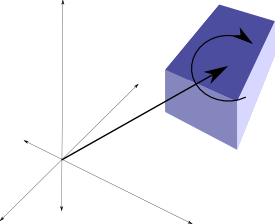
\includegraphics[height=1.4in]{figures/rigidbody.png}
		\end{center}
		
	\column{.5\textwidth}
		\begin{center}
		Can be parameterized by a translation $t$ and a rotation $R$
		
		\vskip15pt
		
		Matrix:
		$\left( \begin{array}{cc}
			R & t \\
			0 & 1 \\
		\end{array} \right)$
		
		\vskip15pt
		$d + {d \choose{2}}$ degrees of freedom
		
		\vskip15pt
		Tangent space: $\mathfrak{so}(d+1)$
		\end{center}
\end{columns}

\vskip10pt
\begin{center}
\bf{Motions of rigid objects $\cong$ paths $q(t) \subset SE(d)$}
\end{center}

\end{frame}

\begin{frame}
\frametitle{Newton's Equations for Rigid Body Dynamics}
Q:Given initial conditions, how do we solve for $q$?
\pause
\vskip5pt
A:High-school physics:
\begin{eqnarray*}
\frac{dq(t)}{dt} & = & \dot{q}(t) \\
M \frac{d\dot{q}(t)}{dt} & = & F(t)
\end{eqnarray*}
\vskip10pt

$F(t)$ is the force vector and $M$ is the mass matrix for the rigid body:
\[ M = \int \limits_{\R^d} \varphi(x) dx \]
\end{frame}

\begin{comment}
\begin{frame}
\frametitle{Multiple rigid bodies}

\end{frame}

\begin{frame}
\frametitle{Lagrangian Mechanics}
Turns physics into an optimization problem.

For each path, $q : \R \to SE(d)$, define a functional
\[ \mathcal{L}(q) = T(q) - U(q) \]
Where $T(q)$ is the total kinetic energy along $q$ and $U$ is the potential energy.

$\mathcal{L}$ measures the work done along $q$

\bf{Physical trajectories correspond to paths of minimal work.}

\end{frame}

\begin{frame}
\frametitle{Rigid Motions in 2D}
For the sake of concreteness, let $d = 2$

Elements of $SE(2)$ are $3 \times 3$ matrices, parameterized by $(\theta, x, y)$:
\[ (\theta, x, y) = \left ( \begin{array}{ccc}
\cos(\theta) & \sin(\theta) & x \\
-\sin(\theta) & \cos(\theta) & y \\
0 & 0 & 1 \\
\end{array} \right) \]
\end{frame}
\end{comment}


\end{document}

